% ****** Start of file apssamp.tex ******
%
%   This file is part of the APS files in the REVTeX 4.1 distribution.
%   Version 4.1r of REVTeX, August 2010
%
%   Copyright (c) 2009, 2010 The American Physical Society.
%
%   See the REVTeX 4 README file for restrictions and more information.
%
% TeX'ing this file requires that you have AMS-LaTeX 2.0 installed
% as well as the rest of the prerequisites for REVTeX 4.1
%
% See the REVTeX 4 README file
% It also requires running BibTeX. The commands are as follows:
%
%  1)  latex apssamp.tex
%  2)  bibtex apssamp
%  3)  latex apssamp.tex
%  4)  latex apssamp.tex
%
\documentclass[%
 reprint,	
%superscriptaddress,
%groupedaddress,
%unsortedaddress,
%runinaddress,
%frontmatterverbose, 
%preprint,
showpacs,
% preprintnumbers,
%nofootinbib,
%nobibnotes,
%bibnotes,
 amsmath,amssymb,
 aps,
 prc,
%prb,
%rmp,
%prstab,
%prstper,
%floatfix,
]{revtex4-1}

\usepackage{graphicx}% Include figure files
\usepackage{dcolumn}% Align table columns on decimal point
\usepackage{bm}% bold math
\usepackage{url}
\usepackage{lipsum}
\usepackage{color}
\usepackage{hyperref}% add hypertext capabilities
\usepackage[mathlines]{lineno}% Enable numbering of text and display math
\usepackage{upgreek}
\usepackage{biolinum}
% \linenumbers\relax % Commence numbering lines

%\usepackage[showframe,%Uncomment any one of the following lines to test 
%%scale=0.7, marginratio={1:1, 2:3}, ignoreall,% default settings
%%text={7in,10in},centering,
%%margin=1.5in,
%%total={6.5in,8.75in}, top=1.2in, left=0.9in, includefoot,
%%height=10in,a5paper,hmargin={3cm,0.8in},
%]{geometry}

% \setcounter{secnumdepth}{5}
\begin{document}

\preprint{APS/123-QED}

\title{Measurement of $\phi(1020)$-meson Production in Au+Au Collisions at ${\sqrt{s_{\rm NN}} = \rm{3\,GeV}}$}% Force line breaks with \\
%\thanks{A footnote to the article title}%

% \author{Ann Author}
% \altaffiliation[Also at ]{Physics Department, XYZ University.}%Lines break automatically or can be forced with \\
% \author{Second Author}%
% \email{Second.Author@institution.edu}
% \affiliation{% Authors' institution and/or address\\ This line break forced with \textbackslash\textbackslash
% }%

\collaboration{STAR Collaboration}
\noaffiliation

\date{\today}% It is always \today, today,
             %  but any date may be explicitly specified

\begin{abstract}


We report on the first measurement of $\phi$-meson production and $\phi/K^-$ ratio in Au+Au collisions at ${\sqrt{s_{\rm NN}} = \rm{3\,GeV}}$ with RHIC/STAR experiment under fixed target configuration. $\phi$-mesons are measured through their hadronic decay channel, $\phi\rightarrow K^+K^-$. The transverse momentum ($p_T$) spectra of $\phi$-mesons and $K^-$ are presented in different centrality and rapidity intervals. The total production yields and $\phi/K^-$ ratio in $4\pi$ acceptance are calculated and compared to thermal model predictions. The grand canonical ensemble (GCE) calculation shows a clear discrepancy from our measurement. Our data favors the canonical ensemble (CE) model with a strangeness correlation length $(r_c   \sim 3.2_{-0.3}^{+0.2} \rm{fm})$ in 0--10\% central Au+Au collisions at ${\sqrt{s_{\rm NN}} = \rm{3\,GeV}}$.


%\begin{description}
%\item[Usage]
%Secondary publications and information retrieval purposes.
%\item[PACS numbers]
%May be entered using the \verb+\pacs{#1}+ command.
%\item[Structure]
%You may use the \texttt{description} environment to structure your abstract; use the optional argument of the \verb+\item+ command to give the category of each item. 
%\end{description}
\end{abstract}

\pacs{25.75.-q, 25.75.Cj}% PACS, the Physics and Astronomy
                             % Classification Scheme.
%\keywords{Suggested keywords}%Use showkeys class option if keyword
                              %display desired
\maketitle

% Chapter one
% \section{Introduction}
% \label{introduction}

Relativistic heavy ion physics is aimed for detail investigation of phase structures of strongly interacting matter, governed by Quantum Chromodynamics (QCD), under extreme high temperature and density conditions. Particle production has been studied to investigate the properties of the produced QCD matter in heavy ion collisions. Strange flavor quark has a unique sensitivity in studying the hot QCD medium in heavy-ion collisions because its mass is comparable to the QCD scale as well as to the temperature of the produced medium. The strange quark dynamics plays an important role in understanding the QCD Equation-of-State particularly at high baryon density region. 

Statistical thermal models has been often used to characterize the thermal properties of the produced system. In these models, Grand Canonical Ensemble (GCE) and Canonical Ensemble (CE) statistical descriptions can be applied to conserved electric charge, baryon number, and strangeness number in order to compute the final state particle yields. Both GCE and CE models are able to describe various particle yields including strange particles produced in heavy-ion collisions at RHIC and LHC at center-of-mass energy ($\sqrt{s_{\rm NN}}$) greater than 7.7\,GeV. It is been argued that at lower energies, strangeness number need to be conserved on the event-by-event basis described by the CE, which leads to a reduction in the yields of hadrons with non-zero strangeness number (``Conanical Suppression").

$\phi(1020)$ meson is the lightest bound state of $s\bar{s}$ with zero net strangeness number. The $\phi$ meson production in elementary collisions is suppressed compared to other strange hadrons due to the QCD Okubo-Zweig-Iizuka rule. So with the GCE description, the $\phi/K^-$ ratio is expected to fall off when the collision energy decreases. With the CE description, $\phi$ meson production is not affected by the event-by-event strangeness number conservation, unlike other strange hadrons ($K^-$, $\Lambda$ etc.). Therefore, the $\phi/K^-$ ratio is expected to increase with decreasing collision energy in models using the CE treatment for strangeness. The $\phi/K^-$ ratio offers a unique test to scrutinize thermodynamic properties of strange quarks in the hot and dense QCD environment.

Measurements from AGS, SPS, RHIC and LHC show that the $\phi/K^-$ ratio in heavy-ion collisions stays remarkably flat ($\sim$0.15) at collisions energy $\sqrt{s_{\rm NN}}>$5\,GeV. Recent measurements of the $\phi/K^-$ ratio in heavy-ion collisions at the collision energies below the $\phi$ production threshold in NN collisions ($\sim$2.9\,GeV) from HADES and FOPI Collaborations show a hint of relative enhancement compared to that from high energies at RHIC and LHC, %These enhancement were observed both in Au+Au collisions and also in the lighter system such as Ni+Ni, Ar+KCl and Al+Al at low energies.
indicative of the necessity of the CE description for strangeness production at these energies. In the CE model, a correlation length parameter $r_c$ is often used to characterize the volume size to account for the strangeness local conservation, which remains large uncertain with the existing measurements.
%The grand canonical ensemble (GCE) statistical model shows a discrepancy with the measured data while the calculations from canonical ensemble (CE) with different strangeness correlation length ($r_c$) can reasonable reproduce this feature. In the GCE, the strangeness was conserved in average for the collision system, while the $r_c$ parameter in CE model corresponding to the strangeness local conserved volume size. Due to the uncertainties in the current measurements, a solid determination on the $r_c$ and distinguish those different models are still missing. 
The RHIC Beam Energy Scan phase-II program including both collider and fixed target setups with the STAR experiment covers a center-of-mass energy range of 3.0--19.6\,GeV. This offers us a great opportunity to conduct precise measurement of the energy dependence of $\phi/K^-$ ratio at low collision energies, which is crucial in order to understand the strangeness dynamics as well as the medium properties at high baryon density regions in QCD.
%to 7.7 GeV which can map the unmeasured cms range to have a better constrain on the model calculations and understanding the strangeness production mechanisms~\cite{}.

The dataset used in this analysis consists of Au+Au collision at fixed-target (FXT) mode with ${\sqrt{s_{\rm NN}} = \rm{3\,GeV}}$ collected in the 2018 RHIC run. The main detectors used are the Time Projection Chamber (TPC), the Time of Flight (TOF) detector and the Beam-Beam Counter (BBC). The trigger system is provide by the BBC detector, while the tracking and particle identification by TPC and TOF. Events are selected with the offline reconstructed collision vertex within 1.5 cm of the target centers along the beam direction. Approximately 2.6$\times 10^{8}$ minimum bias (MB) triggered events with 0--80\% centrality pass the selection criteria and are used in this analysis. 

\textcolor{red}{need to add some description on the fixed target}

\textcolor{red}{need to describe how the centrality is determined}

The $\phi$-mesons are reconstructed via the hadronic decay channel $\phi\rightarrow K^+K^-$ with a branching ratio ($B.R.$) of 49.2\%~\cite{pdg}. Charged kaon tracks are reconstructed with the TPC in a 0.5 T uniform magnetic field. The TPC tracks are required to contain at least 20 TPC hits (out a maximum of 45) to ensure a good tracking and avoid track splitting. Kaons tracks are identified via a combination of the ionization energy loss ($dE/dx$) measurement with the TPC and the time-of-flight ($tof$) measurement with the TOF detector which have been extensively used in many prior STAR analyses. Due to the charge asymmetry for the particle yields at ${\sqrt{s_{\rm NN}} = \rm{3\,GeV}}$, a smaller yield for $K^-$ means a relative higher contaminations, thus a strict PID requiring both TPC and TOF are implemented. Both the TPC and TOF detectors have full azimuthal coverage with a pseudo-rapidity range of 0$<$\,$\eta$\,$<$\,1.88 for TPC and 0$<$\,$\eta$\,$<$\,1.5 for TOF at FXT mode~\cite{TPC,TOF}.



\begin{figure}
\centering
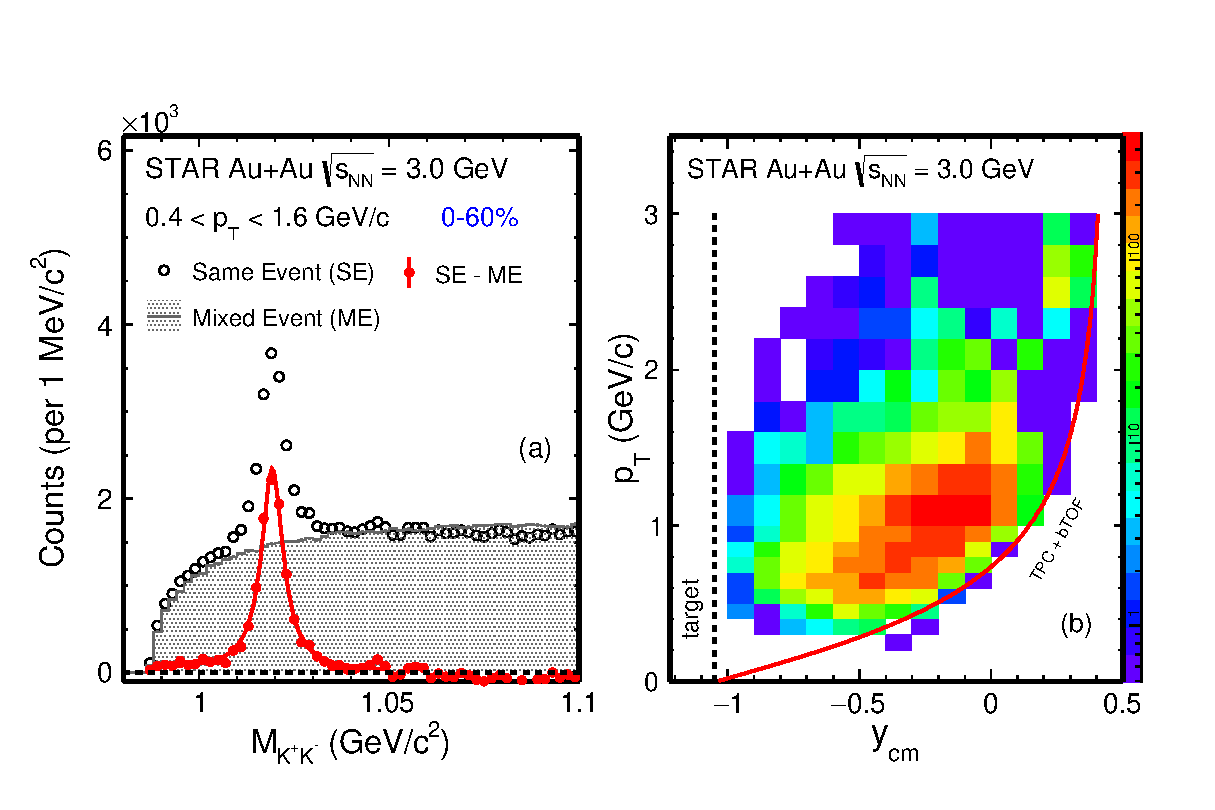
\includegraphics[width=0.52\textwidth]{fig/fig1_signal.eps}
  \caption{(a) Invariant mass distributions of $K^+K^-$ pairs with the pair $p_T$ of 0.4--1.6\,GeV/$c$ in 0-60\% Au+Au collisions at ${\sqrt{s_{\rm NN}} = \rm{3\,GeV}}$. Black open circles represent the same-event unlike-sign distribution. The grey shaded histogram represents the normalized mix-event unlike-sign distribution that are used to estimate the combinatorial background. The red solid circles depict the $\phi$-meson signals obtained by subtracting the mixed-event background from the same-event distribution. (b) Reconstructed $\phi$-meson acceptance $p_T$ vs. rapidity in the center-of-mass frame ($y_{\rm cm}$) in Au+Au collisions at ${\sqrt{s_{\rm NN}} = \rm{3\,GeV}}$. The dotted line at $y_{\rm cm}$ indicates the target rapidity location and the solid red line indicate the acceptance edge for charged kaon tracks selected by TPC + barrel TOF (bTOF).}
\label{fig:phiSignal} 
\end{figure}


Figure~\ref{fig:phiSignal} left shows example of the invariant mass distributions of $K^+K^-$ pairs in the $p_{T}$ region of 0.4--1.6 GeV/$c$ for 0--60\% centrality collisions. The combinatorial background is estimated with the mixed-event (ME) technique in which $K^+$ and $K^-$ from different events of similar characteristics (centrality, event plane angle) are paired. The mixed-event spectra are normalized to the same-event (SE) distributions in the mass range of 1.04--1.08\,GeV/$c^2$. After the subtraction of the combinatorial background, the remainder distributions are shown as red solid circles in the bottom. The reminder $K^+K^-$ invariant mass distributions are fit to a Breit-Wigner for the signal plus a linear function represent the remaining correlated background. The $\phi$-meson raw yields are extracted from the Breit-Wigner function fit results within the corresponding mass windows.



The reconstructed $\phi$-meson acceptance ($p_T$ vs. $y_{cm}$) is shown on the right panel of Fig.~\ref{fig:phiSignal}. The target is located around $y_{cm}$ = -1.05 whereas the convention use the beam-going direction as the positive direction. The red curve represent the TPC and TOF acceptance edges where the reconstructed data covers most of the one-side mid-rapidity ranges for $\phi$-meson.


The reconstructed $\phi$-meson and $K^-$ raw yields are calculated in each centrality and $p_{T}$ bin within each rapidity slices. The corrected $\phi$-meson and $K^-$ production invariant yields are then calculated using the following formula:
\begin{equation}
  \begin{aligned}
 \frac{d^2N}{2\pi p_{T}dp_{T}dy} = \frac{1}{\rm B.R.} \times \frac{N^{\rm raw}}{N_{\rm evt} 2\pi p_{T}\Delta p_{T}\Delta y} \times \frac{1}{\varepsilon_{\rm TPC}\times\varepsilon_{\rm PID}},
  \end{aligned}
\label{equ:invariantyield}
\end{equation}
where B.R. is the corresponding decay branching ratio, $N^{\rm raw}$ is the reconstructed raw counts, $N_{\rm evt}$ is the total numbers of events in corresponding centralities. The raw yields are corrected for the TPC acceptance and tracking efficiency - $\varepsilon_{\rm TPC}$ and the particle identification efficiency - $\varepsilon_{\rm PID}$.


The uncertainty of the raw yield extraction is estimated by changing the raw yield counting method from the fit (breit-wigner function for $\phi$-meson $K^+K^-$ invMass pair distribution) to histogram bin counting. The maximum difference between these scenarios is then converted to the standard deviation and added to the systematic uncertainties. The contribution varies by $p_T$, rapidity and centrality since the statistics is correlated, but the overall contribution is less than 5\% for the total cross section. The uncertainty of the TPC acceptance and efficiency correction $\varepsilon_{\rm TPC}$ is estimated via the standard procedure in STAR by comparing the TPC track distributions between real data and the embedding data, then by varying the track quality cuts such as the nHits fit point and dca used for tracking. After correct the corresponding efficiency for each scenarios, the difference is added to the systematic uncertainties. This contribution for $\phi$-meson is about 13-16\% and 4-5\% for $K^-$ in the reported 3 centrality species and results to 10-13\% for the measured $\phi/K^-$ ratio. The uncertainty of the PID efficiency correction is estimated in a similar way by varying the PID selection cuts such as the TPC $n\sigma_{K}$ and TOF $1/\beta$ and then convoluting to the final corrected yield. This part have relative small contribution less than 2-3\%. For the $p_T$ integrated yield (down to 0 GeV/$c$) measurement, limited by the acceptance, one important systematic source coming from the extrapolation. We estimate this by varying several different fitting functions including levy, blast wave, $m_T$-exponential, $p_T$-exponential, $p_T$-gaussian and etc~\cite{PhysRevC.79.034909}. The maximum difference between these scenarios to the default one ($m_T$-exponential) is then converted and quoted as the systematic source. This contribution for $\phi$-meson is about 14-17\% and 5-7\% for $K^-$. For each individual $\phi$-meson and $K^-$ measurement, some of the uncertainties are correlated or partially correlated (e.g. TPC and PID). Thus for the $\phi/K^-$ ratio measurement, in order to avoid the correlation we vary the above cuts simultaneously for $\phi$-meson and $K^-$, then quote the final ratio difference directly as the systematic uncertainties.


\begin{figure}
\centering
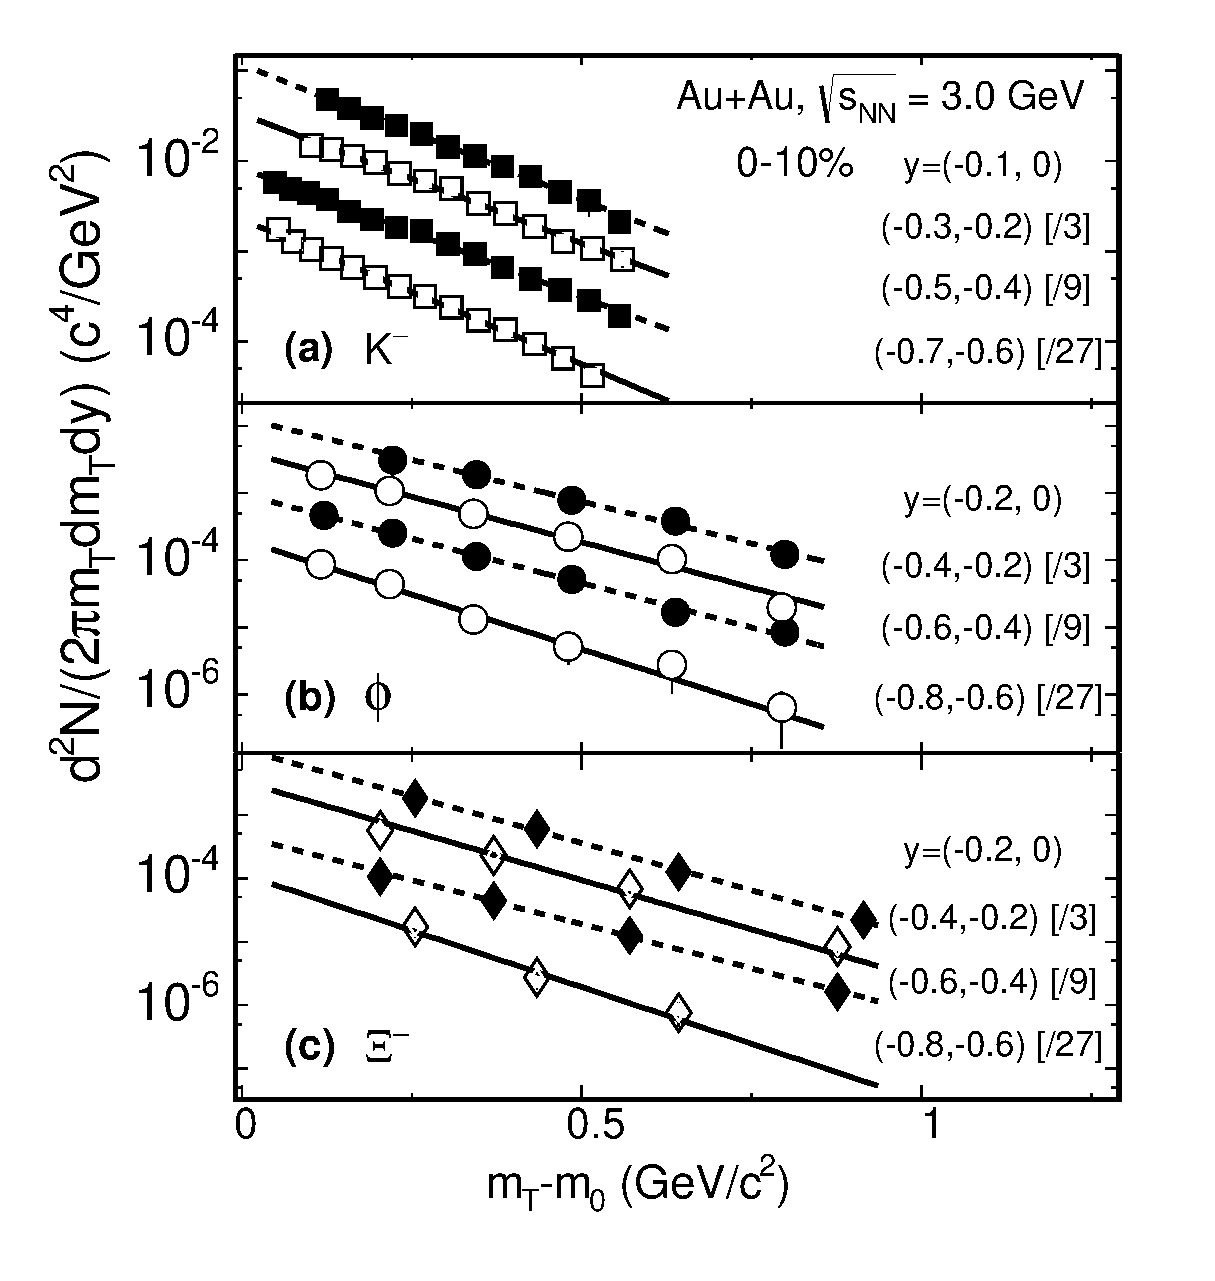
\includegraphics[width=0.41\textwidth]{fig/fig2_h_mT_spectra_phiMeson.eps}
  \caption{ $\phi$-meson and $K^-$ invariant yield as a function of transverse kinetic energy ($m_T-m_0$) for various rapidity regions in 0--10\% central Au+Au collisions at ${\sqrt{s_{\rm NN}} = \rm{3\,GeV}}$. Solid and dashed black lines depict exponential function fits to the measured data points.}
\label{fig:phimTSpectra} 
\end{figure}


\begin{table*}
\centering{
  \caption{$\phi$ and $K^-$ integral yield and $T_{eff}$ as well as $\phi/K^-$ratios for given centrality classes. The first given error corresponds to the statistical, the second to the systematic error.}
\begin{tabular}{cccccc} \hline \hline
  \hspace{0.8cm} & \langle\phi\rangle \ [10^-3/evt]  & \phi\-T_{eff} \ [MeV] & \langle K^-\rangle \ [10^-2/evt] & K^-\-T_{eff} \ [MeV] & \langle\phi\rangle/\langle K^-\rangle   \\ \hline
  0--10\%   & $19.9\pm1.4\pm4.1$  & 176\pm10\pm13  & 8.67\pm0.02\pm 0.53  & 158\pm3\pm3 & $0.23\pm0.02\pm0.04$ \\
  10--40\%  & $8.36\pm0.4\pm1.8$  & 161\pm9\pm10   & 3.41\pm0.01\pm 0.21  & 145\pm2\pm3 & $0.25\pm0.01\pm0.05$ \\
  40--60\%  & $2.68\pm0.2\pm0.6$  & 147\pm9\pm16   & 0.78\pm0.01\pm 0.06  & 109\pm4\pm4 & $0.34\pm0.03\pm0.07$ \\ \hline \hline
\end{tabular}
}
\label{table:singlecut} 
\end{table*}

\begin{figure*}
\centering
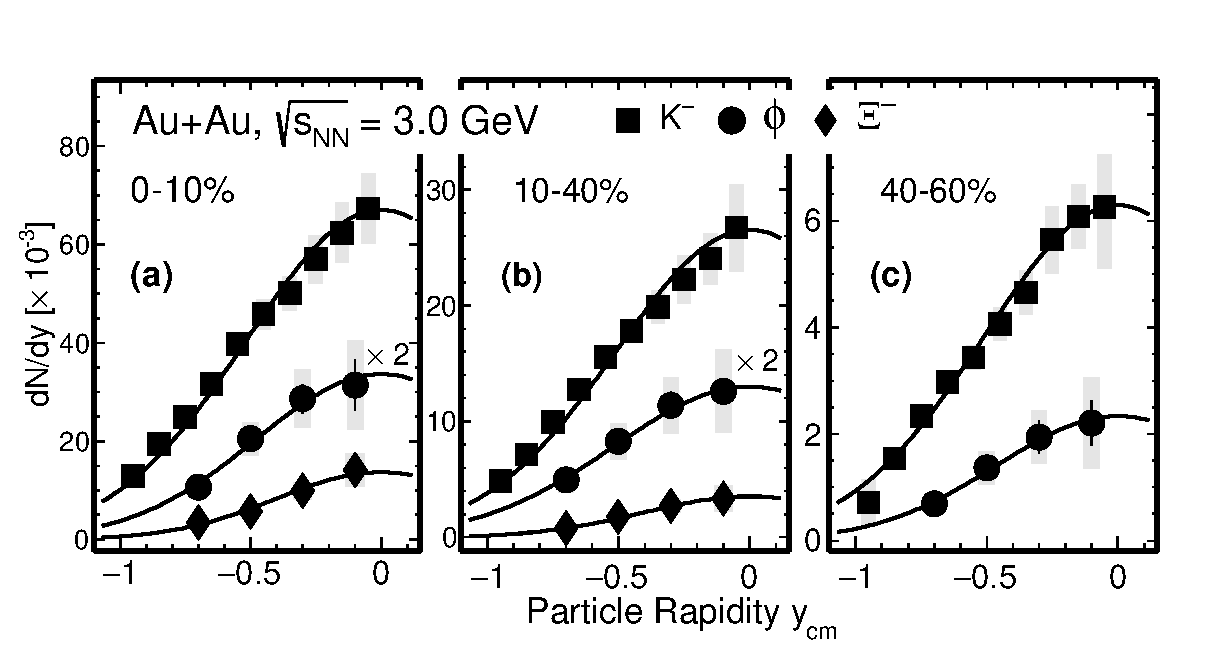
\includegraphics[width=0.8\textwidth]{fig/fig3_dndy.eps}
  \caption{ Rapidity distributions of $K^-$ (squares) and $\phi$-meson (circles) $p_T$-integrated yields $dN/dy$ in 0--10\% (a), 10--40\% (b) and 40--60\% (c) Au+Au collisions at ${\sqrt{s_{\rm NN}} = \rm{3\,GeV}}$. The full symbols show the measured data, while the open ones are reflected data with respect to $y=0$ in the center-of-mass frame. Solid lines depict Gaussian function fits to the data points.}
\label{fig:phiYSpectra} 
\end{figure*}

Figure~\ref{fig:phimTSpectra} shows example of the efficiency--corrected $\phi$-meson and $K^-$ invariant yield as a function of transverse kinetic energy ($m_T-m_0$) for various rapidity regions in 0--10\% central Au+Au collisions at ${\sqrt{s_{\rm NN}} = \rm{3\,GeV}}$. $\phi$-meson and $K^-$ spectra in some rapidity species are scaled with arbitrary factors indicated on the figure for clarity. Dashed and solid lines depict fits to the spectra with the default $m_T$ exponential function to extrapolate the unmeasured $p_T$ ranges. The fitted inverse slope parameters indicate harder spectra for $\phi$-meson compare to $K^-$, and the inverse slope parameters gradually decrease from mid-rapidity to forward rapidity and follow well with the $T_{\rm eff}/\cosh(y_{cm})$ distribution. $T_{eff}$ is extracted to ($176\pm10_{stat}\pm13_{sys}$) MeV for $\phi$ meson in 0--10\% central collisions and following the trends as the other experimental~\cite{2018403,PhysRevC.80.025209,PhysRevC.78.044907}.


The rapidity density distributions are obtained for $\phi$-meson and $K^-$ by integral the measured data points in Fig.~\ref{fig:phimTSpectra} and use the exponential fits for the extrapolation to the unmeasured phase space. The rapidity distributions are displayed in Fig.~\ref{fig:phiYSpectra} for Au+Au collisions at ${\sqrt{s_{\rm NN}} = \rm{3\,GeV}}$ for three different centralities. The full symbols show the measured data, while the open ones are reflected data with respect to $y=0$ in the center-of-mass frame. Solid lines depict Gaussian function fits to the data points and used to extrapolate the unmeasured rapidity windows. In the fitting procedure, the center of the Gaussian was fixed at zero to take into account the symmetry of the reaction. By integral the measured rapidity data point in Fig.~\ref{fig:phiYSpectra} and the Gaussian fit for the extrapolation, the multiplicity for $\phi$-meson and $K^-$ per triggered event were obtained respectively.


The excitation function of $\phi/K^-$ ratio is depicted in Fig.~\ref{fig:phi2Kratio} as a function of collision energy $\sqrt{s_{\rm NN}}$, including AGS, SPS for higher energies and SIS for lower energies. The colored full symbols show these measurements in three centrality bins in Au+Au collisions at ${\sqrt{s_{\rm NN}} = \rm{3\,GeV}}$. The measured ratio is about ($0.230\pm0.016_{stat}\pm0.042_{sys}$) for 0--10\% central , ($0.245\pm0.012_{stat}\pm0.048_{sys}$) for 10--40\% and ($0.344\pm0.026_{stat}\pm0.072_{sys}$) for 40--60\% centrality collisions.
\textcolor{red}{can we just tabulate the dNdy of K-, $\phi$ and $\phi/K^-$ ratio in different centrality bins?}
Which is significantly ($5\sigma$) above than 0 and slightly higher than the approximately constant value ($\approx0.15$) at high energies for $\sqrt{s_{\rm NN}}\geqslant$ 5\,GeV. The measured data points follow well with the energy dependence trend, which the value gradually increase with the energy descent at low $\sqrt{s_{\rm NN}}$. Our measured data points confirmed this enhancement observation which limited by the precision in the previous measurements. There is no clear hint of centrality dependence in the 0--10\% and 10--40\% centralities for the ratio measurement, while for the most peripheral collisions 40--60\% observed a larger values within uncertainties, which is consistent with the picture as measured in $p+p$ collisions~\cite{PhysRevC.77.015204}.


\begin{figure}
\centering
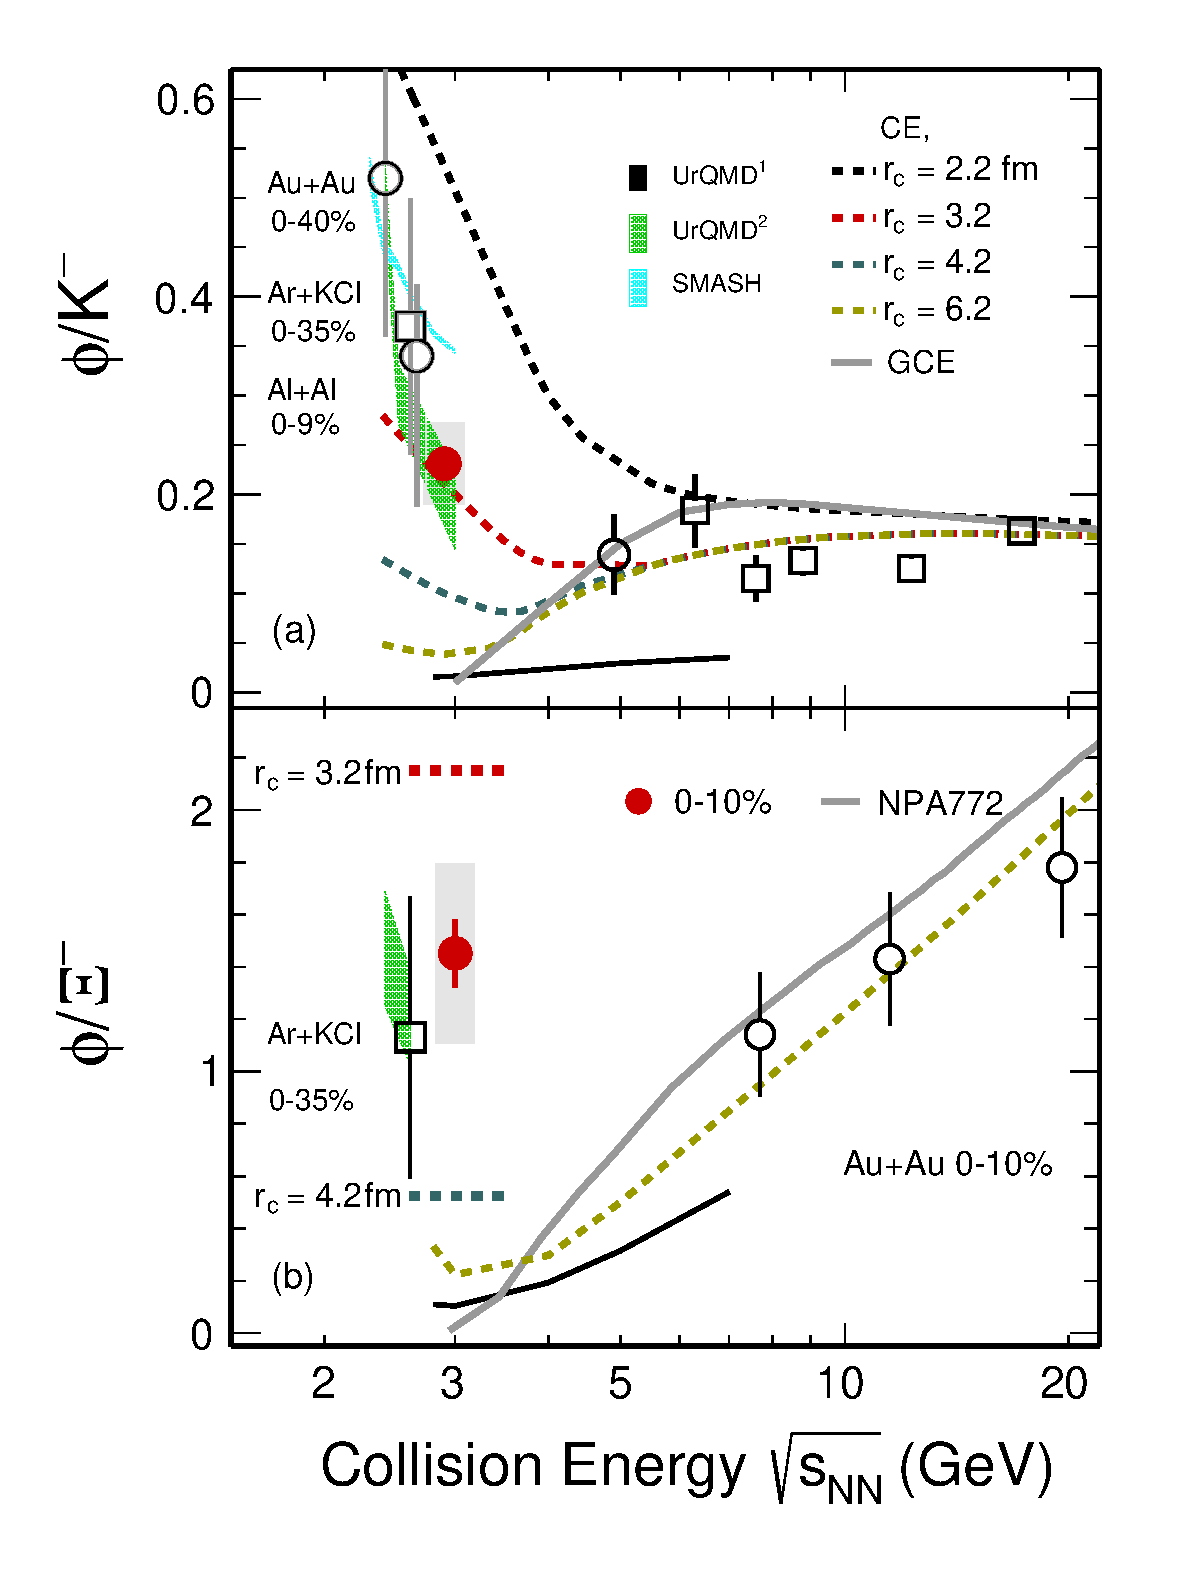
\includegraphics[width=0.41\textwidth]{fig/fig4_phi_over_kminus_zoomin.eps}
  \caption{ $\phi/K^-$ ratio as a function of collision energy $\sqrt{s_{\rm NN}}$. The colored full symbols show these measurements in three centrality bins, whereas the other data points represented by different markers from various energies and collision systems. The red arrow depict the $\phi$-meson production threshold in proton-proton collisions. The grey solid line represents a thermal model calculation based on Grand Canonical Ensemble (GCE) while the dotted lines depict calculations based on Canonical Ensemble (CE) with four different parameters of strangeness correlation radius ($r_c$). The blue and red bands show transport model calculations from UrQMD and SMASH, respectively.}
\label{fig:phi2Kratio} 
\end{figure}


Despite the different collision system and size including Au+Au, Ni+Ni, Ar+KCl and Al+Al, both of them observed substantially larger ratio in the low energy compare to high energy. Various curves in the Fig.~\ref{fig:phi2Kratio} represent the predictions from several models calculation. The grand canonical ensemble using the chemical freeze-out parameters derived from the fits of experimental data at mid-rapidity with details in~\cite{ANDRONIC2006167}. The strangeness ($\mu_s$) is conserved on average in GCE, where the model does not contain strangeness suprression factor which accounts for the non-equilibration in the strangeness sector. The model reproduces well for the AGS data point, while slightly deviate from the SPS measurements, despite the model calculations are for midrapidity yield and the experimental measurements are for total multiplicity. It's clear that the model failed to describe the data at low energies including our new measurements at ${\sqrt{s_{\rm NN}} = \rm{3\,GeV}}$, which may indicate the thermal particle phase-space at low energies is far from the GCE limit and the local treatment of strangeness conservation is crucial. In the canonical approach, the correlation length $r_c$ related to a reduction of the particle production phase space inside which the production of the open strangeness is canonically conserved. There are 4 different $r_c$ calculations in Fig.~\ref{fig:phi2Kratio}, with a large $r_c$ = 6.2\,fm, the CE calculation gives approximately results as the GCE calculation. Assuming a linear interpolation with the $r_c$ calculations, and taking into account the statistics and systematic uncertainties of the measured data, our result favors $(r_c  \sim 3.2_{-0.3}^{+0.2} \rm{fm})$ in 0--10\% , $(r_c  \sim 3.2_{-0.3}^{+0.1} \rm{fm})$ in 10--40\% and $(r_c  \sim 2.7_{-0.3}^{+0.3} \rm{fm})$ in 40--60\% centrality Au+Au collisions at ${\sqrt{s_{\rm NN}} = \rm{3\,GeV}}$. Note, the calculation using $r_c = 1.2 \rm{fm}$ is consistent with the measured $\phi/K^-$ ratio in $p+p$ collisions at ANKE~\cite{PhysRevC.80.025209} which is consistent with our centrality dependence trend.

The transport models such as Ultra-relativistic Quantum Molecular Dynamics (UrQMD) are widely used in the high baryon density range to study properties of the produced dense matter. In the model~\cite{Steinheimer_2015}, new decay channels from high mass baryon resonance to $\phi$ and $\Xi^-$ are deployed. The relevant decay branching fraction was determined by fitting the experiment data in elementary proton-proton collisions~\cite{PhysRevC.77.015204}. From the comparison in Fig.~\ref{fig:phi2Kratio}, the UrQMD nicely reproduced the data points at low ${\sqrt{s_{\rm NN}}}$ including our new measurement, while clearly underestimate the measurements for high $\sqrt{s_{\rm NN}}\geqslant 5 GeV$. Another hadronic transport approach called Simulating Many Accelerated Strongly-interacting Hadrons (SMASH) recently has attempted to incorporate the newest available experimental data from both elementary hadronic cross section and dilepton invariant mass spectra to constrain the resonance branching ratios. The $\phi/K^-$ ratio was reasonable reproduced along the low ${\sqrt{s_{\rm NN}}}$ range, but note here each individual ($\phi$, $K^-$) transverse mass spectra predicted in SMASH overestimated the real measurement in Au+Au collisions at HADES which suggest a strangeness-suppressing in-medium effect may be missing.

In summary, we report the first measurement of $\phi(1020)$ meson production and $\phi/K^-$ ratio in Au+Au collisions at ${\sqrt{s_{\rm NN}} = \rm{3\,GeV}}$ with the STAR experiment at RHIC. The measured $\phi/K^-$ ratio is about $5\sigma$ larger than zero in 0--10\% and 10--40\% centrality collisions. The GCE calculation clearly underestimate the measured data, while our measurements favor the CE calculation with $(r_c \sim 3.2_{-0.3}^{+0.2} \rm{fm})$ in 0--10\% central Au+Au collisions. The transport models including the resonance decays can reasonable describe the ratio in low energies. Our data are expected to offer significant constrains towards the understanding of the strangeness production mechanisms and the EoS of the nuclear matter produced in the high baryon density region.



% Chapter acknowledgement
%\section{Acknowledgement}
%\label{acknowledgement}

We thank the RHIC Operations Group and RCF at BNL, the NERSC Center at LBNL, and the Open Science Grid consortium for providing resources and support. This work is supported in part by the Office of Nuclear Physics within the U.S. DOE Office of Science, the U.S. National Science Foundation, the Ministry of Education and Science of the Russian Federation, National Natural Science Foundation of China, Chinese Academy of Science, the Ministry of Science and Technology of China and the Chinese Ministry of Education, the National Research Foundation of Korea, GA and MSMT of the Czech Republic, Department of Atomic Energy and Department of Science and Technology of the Government of India; the National Science Centre of Poland, National Research Foundation, the Ministry of Science, Education and Sports of the Republic of Croatia, RosAtom of Russia and German Bundesministerium f{\"u}r Bildung, Wissenschaft, Forschung and Technologie (BMBF) and the Helmholtz Association.

\bibliography{phi3GeV}

\end{document}
%
% ****** End of file apssamp.tex ******
